% -*- latex -*-
%%%%%%%%%%%%%%%%%%%%%%%%%%%%%%%%%%%%%%%%%%%%%%%%%%%%%%%%%%%%%%%%
%%%%%%%%%%%%%%%%%%%%%%%%%%%%%%%%%%%%%%%%%%%%%%%%%%%%%%%%%%%%%%%%
%%%%
%%%% This text file is part of the source of 
%%%% `Parallel Programming in MPI and OpenMP'
%%%% by Victor Eijkhout, copyright 2012-9
%%%%
%%%% mpi-onesided.tex : about onesided communication
%%%%
%%%%%%%%%%%%%%%%%%%%%%%%%%%%%%%%%%%%%%%%%%%%%%%%%%%%%%%%%%%%%%%%
%%%%%%%%%%%%%%%%%%%%%%%%%%%%%%%%%%%%%%%%%%%%%%%%%%%%%%%%%%%%%%%%

\index{communication!one-sided|(}
\index{target!active synchronization|see{active target synchronization}}
\index{target!passive synchronization|see{passive target synchronization}}

Above, you saw  point-to-point operations of the two-sided type:
they require the co-operation of a sender and
receiver. This co-operation could be loose: you can post a receive
with \indexmpishow{MPI_ANY_SOURCE} as sender, but there had to be both a send and
receive call. In this section, you will see one-sided communication 
routines where a process
can do a `put' or `get' operation, writing data to or reading it from
another processor, without that other processor's involvement.

In one-sided MPI operations, also known as \acf{RDMA} or 
\acf{RMA} operations, there
are still two processes involved: the \indexterm{origin}, which is the
process that originates the transfer, whether this is a `put' or a `get',
and the \indexterm{target} whose
memory is being accessed. Unlike with two-sided operations, the target
does not perform an action that is the counterpart of the action on the origin.

That does not mean that the origin can access arbitrary data on the target
at arbitrary times. First of all, one-sided communication in MPI
is limited to accessing only a specifically declared memory area on the target:
the target declares an area of
user-space memory that is accessible to other processes. This is known
as a \indexterm{window}. Windows limit how origin processes can access
the target's memory: you can only `get' data from a window or `put' it
into a window; all the other memory is not reachable from other processes.

The alternative to having windows is to use \indexterm{distributed shared memory}
or \indexterm{virtual shared memory}: memory is distributed but acts as if
it shared. The so-called \acf{PGAS} languages such as \ac{UPC} use this model.
The MPI \ac{RMA} model makes it possible to 
lock a window which makes programming slightly more cumbersome, but the
implementation more efficient.

Within one-sided communication, MPI has two modes: active RMA and
passive RMA. In \indextermsub{active}{RMA}, or \indexterm{active target synchronization},
the target sets boundaries on the time period (the `epoch')
during which its window can be accessed.
The main advantage
of this mode is that the origin program can perform many small transfers, which are
aggregated behind the scenes. Active RMA acts much like asynchronous transfer with a
concluding \indexmpishow{MPI_Waitall}.

In \indextermsub{passive}{RMA}, or \indexterm{passive target synchronization},
the target process puts no limitation on when its window can be accessed.
(\ac{PGAS} languages such as \ac{UPC} are based on this model: data is 
simply read or written at will.)
While 
intuitively it is attractive to be able to write to and read from a target at
arbitrary time,
there are problems. For instance, it requires a remote agent on the target,
which may interfere with execution of the main thread, or conversely it may not be
activated at the optimal time. Passive RMA is also very hard to debug and can lead
to strange deadlocks.

%% McLaren says use an info object

\Level 0 {Windows}
\label{sec:windows}
\index{window|(}

\begin{figure}[ht]
  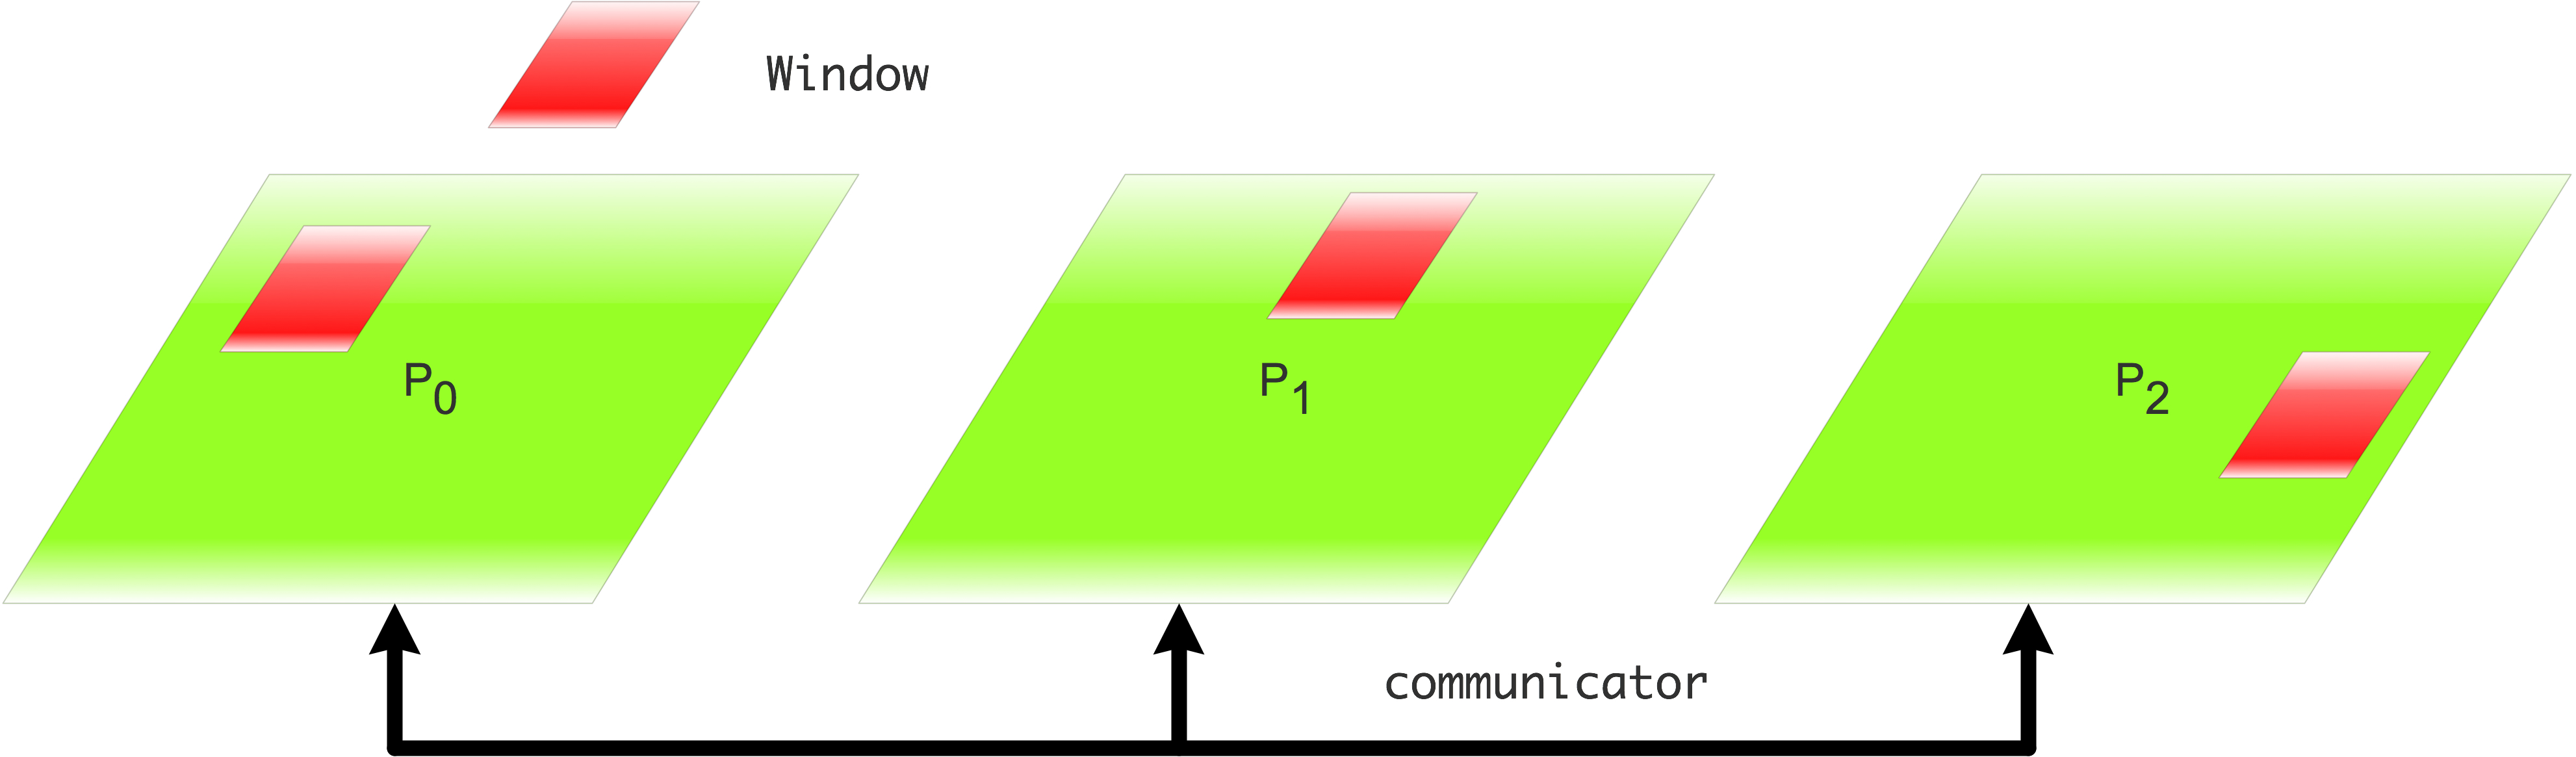
\includegraphics[scale=.1]{one-sided-window}
  \caption{Collective definition of a window for one-sided data access}
  \label{fig:window}
\end{figure}

In one-sided communication, each processor can make an area of memory,
called a \indexterm{window}, available to one-sided transfers.
A~process can put an arbitrary item from its own memory to the
window of another process, or get something from the other process'
window in its own memory.

A window can be characteristized as follows:
\begin{itemize}
\item The window is defined on a communicator, so the create call
  is collective; see figure~\ref{fig:window}. 
\item The window size can be set individually on each process.
  A~zero size is allowed, but since window creation is collective,
  it is not possible to skip the create call.
\item The datatype can also be set individually on each process. This
  makes it possible to use a derived type on one process, for instance
  for copying strided data into a contiguous buffer.
\item The window is the target of data in a put operation, or the
  source of data in a get operation; see figure~\ref{fig:putget}.
\item There can be memory associated with a window, so it needs to be
  freed explicitly.
\end{itemize}

\mpiRoutineRef{MPI_Win}

The typical calls involved are:
\lstset{style=reviewcode,language=C}
\begin{lstlisting}
MPI_Info info;
MPI_Win window;
MPI_Win_allocate( /* size info */, info, comm, &memory, &window );
// do put and get calls
MPI_Win_free( &window );
\end{lstlisting}

\begin{figure}[ht]
  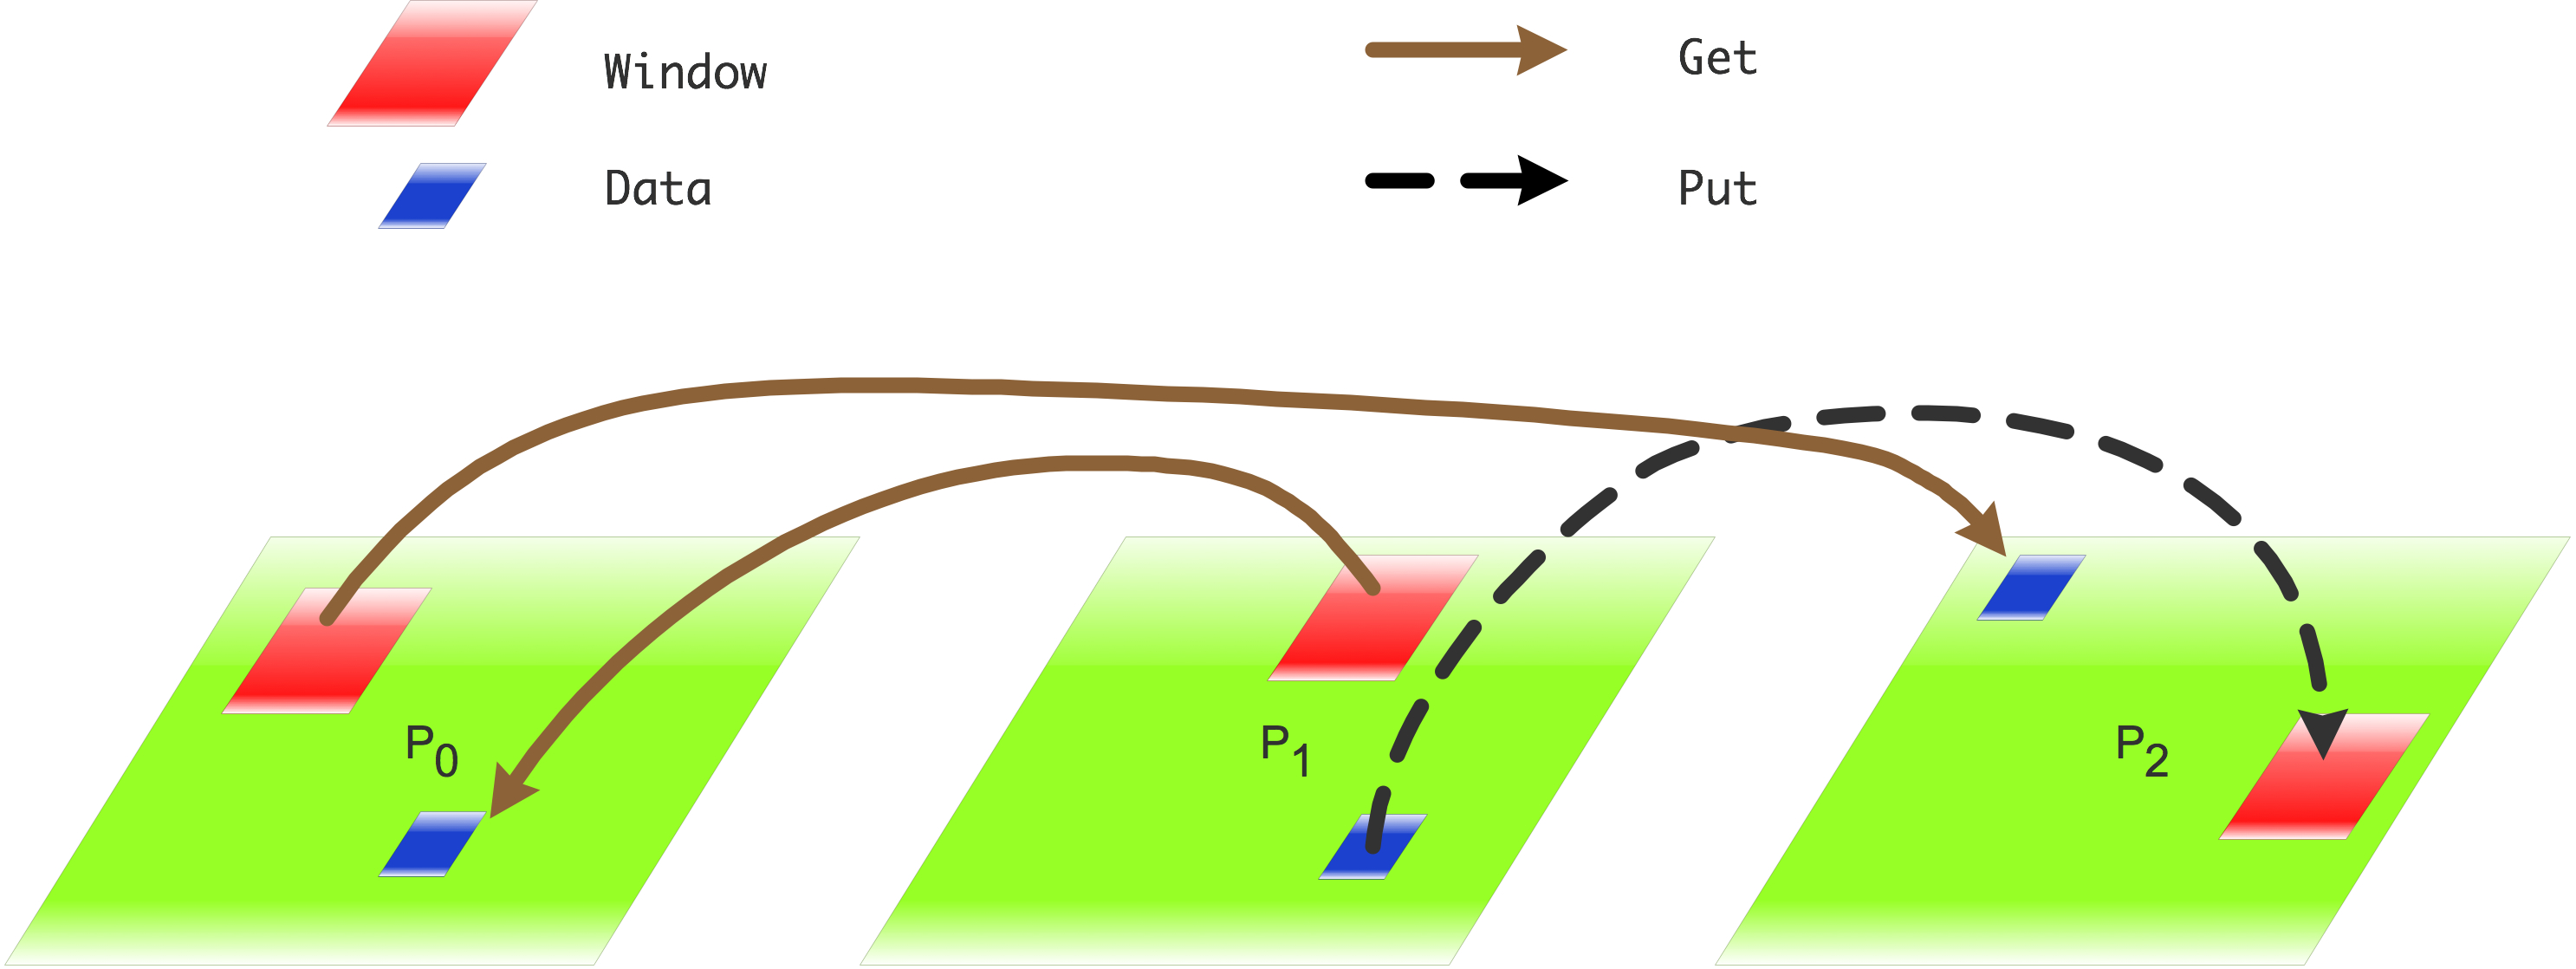
\includegraphics[scale=.1]{one-sided-getput}
  \caption{Put and get between process memory and windows}
  \label{fig:putget}
\end{figure}

\Level 1 {Window creation and allocation}
\label{sec:win-alloc}
\index{window!memory allocation|(}

The memory for a window is ordinary data in user space. There are multiple
ways you can associate data with a window:
\begin{enumerate}
\item You can pass a user buffer to
  \indexmpishow{MPI_Win_create}. This buffer can be an ordinary array,
  or it can be created with \indexmpishow{MPI_Alloc_mem}.
\item You can let MPI do the allocation, so that MPI can perform various
  optimizations regarding placement of the memory. The user code then
  receives the pointer to the data from MPI. This can again be done in two ways:
  \begin{itemize}
  \item Use \indexmpishow{MPI_Win_allocate} to create the data and the
    window in one call, and its variant
  \item If a communicator is on a shared memory (see
    section~\ref{mpi-comm-split-type}) you can create a window in that
    shared memory with \indexmpishow{MPI_Win_allocate_shared}.
  \end{itemize}
\item Finally, you can create a window with
  \indexmpishow{MPI_Win_create_dynamic} which postpones the allocation;
  see section~\ref{sec:mpi-alloc}.
\end{enumerate}

First of all, the create call from a pointer to memory:
%
\mpiRoutineRef{MPI_Win_create}
%
The data array must not be \n{PARAMETER} or \n{static const}.

The size parameter is measured in bytes. In~C this is easily done
with the \indextermtt{sizeof} operator;
for doing this calculation in Fortran, see section~\ref{sec:f-sizeof}.

Next, one can obtain the memory from MPI by using
%
\mpiRoutineRef{MPI_Win_allocate}
%
which has the data pointer as output. Note the \n{void*} in the
C~prototype; it is still necessary to pass a pointer to a pointer:
\lstset{style=reviewcode,language=C}
\begin{lstlisting}
double *window_data;
MPI_Win_allocate( ... &window_data ... );
\end{lstlisting}
The routine \indexmpishow{MPI_Alloc_mem} performs only the allocation
part of \indexmpishow{MPI_Win_allocate}, after which you need to
\indexmpishow{MPI_Win_create}:
%
\mpiRoutineRef{MPI_Alloc_mem}

This memory is freed with
\begin{lstlisting}
MPI_Free_mem()
\end{lstlisting}
These calls reduce to \n{malloc} and \n{free} if there is no special
memory area; SGI is an example where such memory does exist.

There will be more discussion of window memory in section~\ref{sec:win-model}.

\index{window!memory allocation|)}

\Level 0 {Active target synchronization: epochs}
\label{sec:fence}

One-sided communication has an obvious complication over two-sided: if
you do a put call instead of a send, how does the recipient know that
the data is there? This process of letting the target know the state
of affairs is called `synchronization', and there are various
mechanisms for it. First of all we will consider \indexterm{active
  target synchronization}. Here the target knows when the transfer
may happen (the \indextermsub{communication}{epoch}), but does not do
any data-related calls.

In this section we look at the first mechanism,
which is to use a \indexterm{fence} operation:\indexmpi{MPI_Win_fence}
\begin{lstlisting}
MPI_Win_fence (int assert, MPI_Win win)
\end{lstlisting}
This operation is collective on the communicator of the window.
It is comparable to \indexmpishow{MPI_Wait} calls for non-blocking communication.

The use of fences is somewhat complicated. The interval between two fences
is known as an \indextermdef{epoch}.
You can give various hints to the system about this epoch versus the ones
before and after through the \n{assert} parameter.
\begin{lstlisting}
MPI_Win_fence((MPI_MODE_NOPUT | MPI_MODE_NOPRECEDE), win);
MPI_Get( /* operands */, win);
MPI_Win_fence(MPI_MODE_NOSUCCEED, win);
\end{lstlisting}
In between the two fences the window is exposed, and while it is you
should not access it locally. If you absolutely need to access it
locally, you can use an \ac{RMA} operation for that. Also, there can be only one
remote process that does a \n{put}; multiple \n{accumulate} accesses are allowed.

Fences are, together with other window calls, collective operations. That means they 
imply some amount of synchronization between processes. Consider:
\begin{lstlisting}
MPI_Win_fence( ... win ... ); // start an epoch
if (mytid==0) // do lots of work
else // do almost nothing
MPI_Win_fence( ... win ... ); // end the epoch
\end{lstlisting}
and assume that all processes execute the first fence more or less at the same time.
The zero process does work before it can do the second fence call, but all other
processes can call it immediately. However, they can not finish that second fence call
until all one-sided communication is finished, which means they wait for the zero process.
\begin{figure}[ht]
  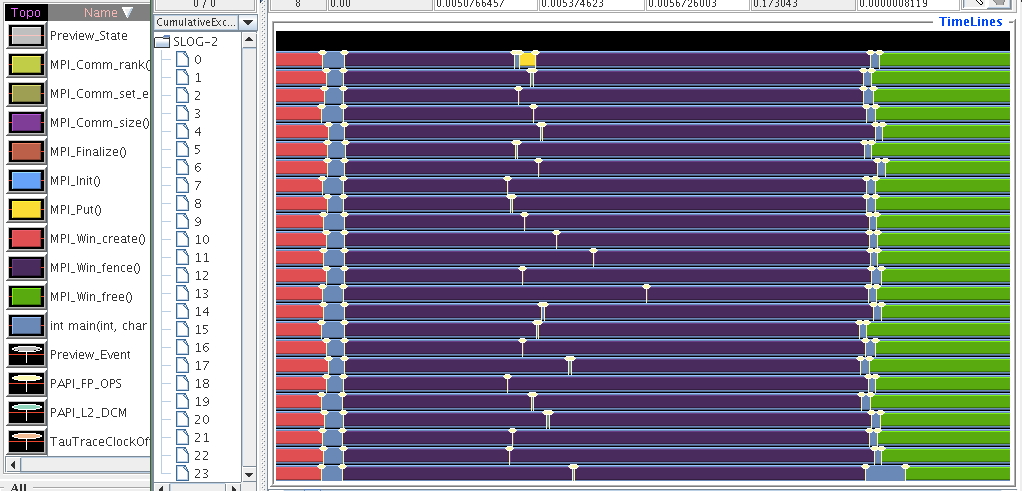
\includegraphics[scale=.4]{graphics/lonestar-twonode-put}%putblock
  \caption{A trace of a one-sided communication epoch where process zero only originates
  a one-sided transfer}
  \label{fig:putblock}
\end{figure}
\cverbatimsnippet[examples/mpi/c/putblock.c]{putblock}

As a further restriction, you can not mix \indexmpishow{MPI_Get} with \indexmpishow{MPI_Put}
or \indexmpishow{MPI_Accumulate} calls in a single epoch. Hence, we can
characterize an epoch as an \indextermsub{access}{epoch} on the
origin, and as an \indextermsub{exposure}{epoch} on the target.

Assertions are an integer parameter: you can combine assertions by
adding them or using logical-or.
The value zero is always correct. For further information, see
section~\ref{sec:mpi-assert}.

%% Local assertions are:
%% \begin{itemize}
%%   \item\indexmpishow{MPI_MODE_NOSTORE} The preceding epoch did not store
%%     anything in this window.
%%   \item\indexmpishow{MPI_MODE_NOPUT} The following epoch will not store
%%     anything in this window.
%% \end{itemize}
%% Global assertions:
%% \begin{itemize}
%%   \item\indexmpishow{MPI_MODE_NOPRECEDE} This process made no \ac{RMA}
%%     calls in the preceding epoch.  
%%   \item\indexmpishow{MPI_MODE_NOSUCCEED} This process will make no
%%     \ac{RMA} calls in the next epoch.
%% \end{itemize}

\index{window|)}

\Level 0 {Put, get, accumulate}
\label{sec:putget}

We will now look at the first three routines for doing one-sided
operations: the Put, Get, and Accumulate call. (We will look at
so-called `atomic' operations in section~\ref{sec:mpi-atomic}.)
These calls are somewhat
similar to a Send, Receive and Reduce, except that of course only one
process makes a call.
Since one process does all the work, its calling sequence contains
both a description of the data on the origin (the calling process) and
the target (the affect other process).

As in the two-sided case, \indexmpishow{MPI_PROC_NULL} can be used as
a target rank.

\Level 1 {Put}

The \indexmpishow{MPI_Put} call can be considered as a one-sided
send. As such, it needs to specify
\begin{itemize}
\item the target rank
\item the data to be sent from the origin, and
\item the location where it is to be written on the target.
\end{itemize}

The description of the data on the origin is the usual trio of
buffer/count/datatype. However, the description of the data on the
target is more complicated. It has a count and a datatype, but instead
of an address it has a
\emph{displacement unit}\index{window!displacement unit} with respect to the
start of the window on the target. This displacement can be given in
bytes, so its type is \indexmpishow{MPI_Aint}, but strictly speaking
it is a multiple of the displacement unit that was specified in the
window definition.

Specifically, data is written starting at
\[ \mathtt{window\_base} + \mathtt{target\_disp}\times \mathtt{disp\_unit}. \]

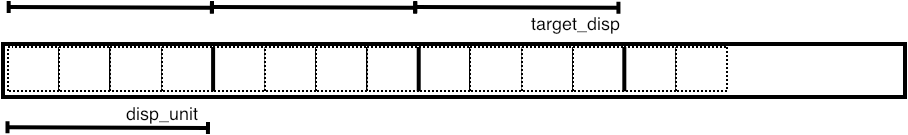
\includegraphics[scale=.4]{windowdisp}

\mpiRoutineRef{MPI_Put}

\begin{fortrannote}
  The \n{disp_unit} variable is declared as 
\lstset{style=reviewcode,language=Fortran} %pyskip
\begin{lstlisting}
integer(kind=MPI_ADDRESS_KIND) :: displacement
\end{lstlisting}
\lstset{style=reviewcode,language=C} %pyskip
  Specifying a literal constant, such as~\n{0}, can lead to bizarre
  runtime errors.
\end{fortrannote}

Here is a single put operation. Note that the window create and window fence calls
are collective, so they have to be performed on all processors
of the communicator that was used in the create call.
\cverbatimsnippet[examples/mpi/c/putblock.c]{putblock}

\begin{exercise}
  \label{ex:rightput}
  Revisit exercise~\ref{ex:serialsend} and solve it using
  \indexmpishow{MPI_Put}.
\end{exercise}

\begin{exercise}
  \label{ex:randomput}
  Write code where process~0 randomly writes in the window on 1~or~2.
  %\cverbatimsnippet{randomputskl}
\end{exercise}

\Level 1 {Get}

The \indexmpishow{MPI_Get} call is very similar.
%
\mpiRoutineRef{MPI_Get}
%
Example:
%
\cverbatimsnippet[examples/mpi/c/getfence.c]{getfence}
%
We make a null window on processes that do not participate.
%
\pverbatimsnippet{getfencep}

\Level 1 {Put and get example: halo update}

\begin{wrapfigure}{r}{3in}
  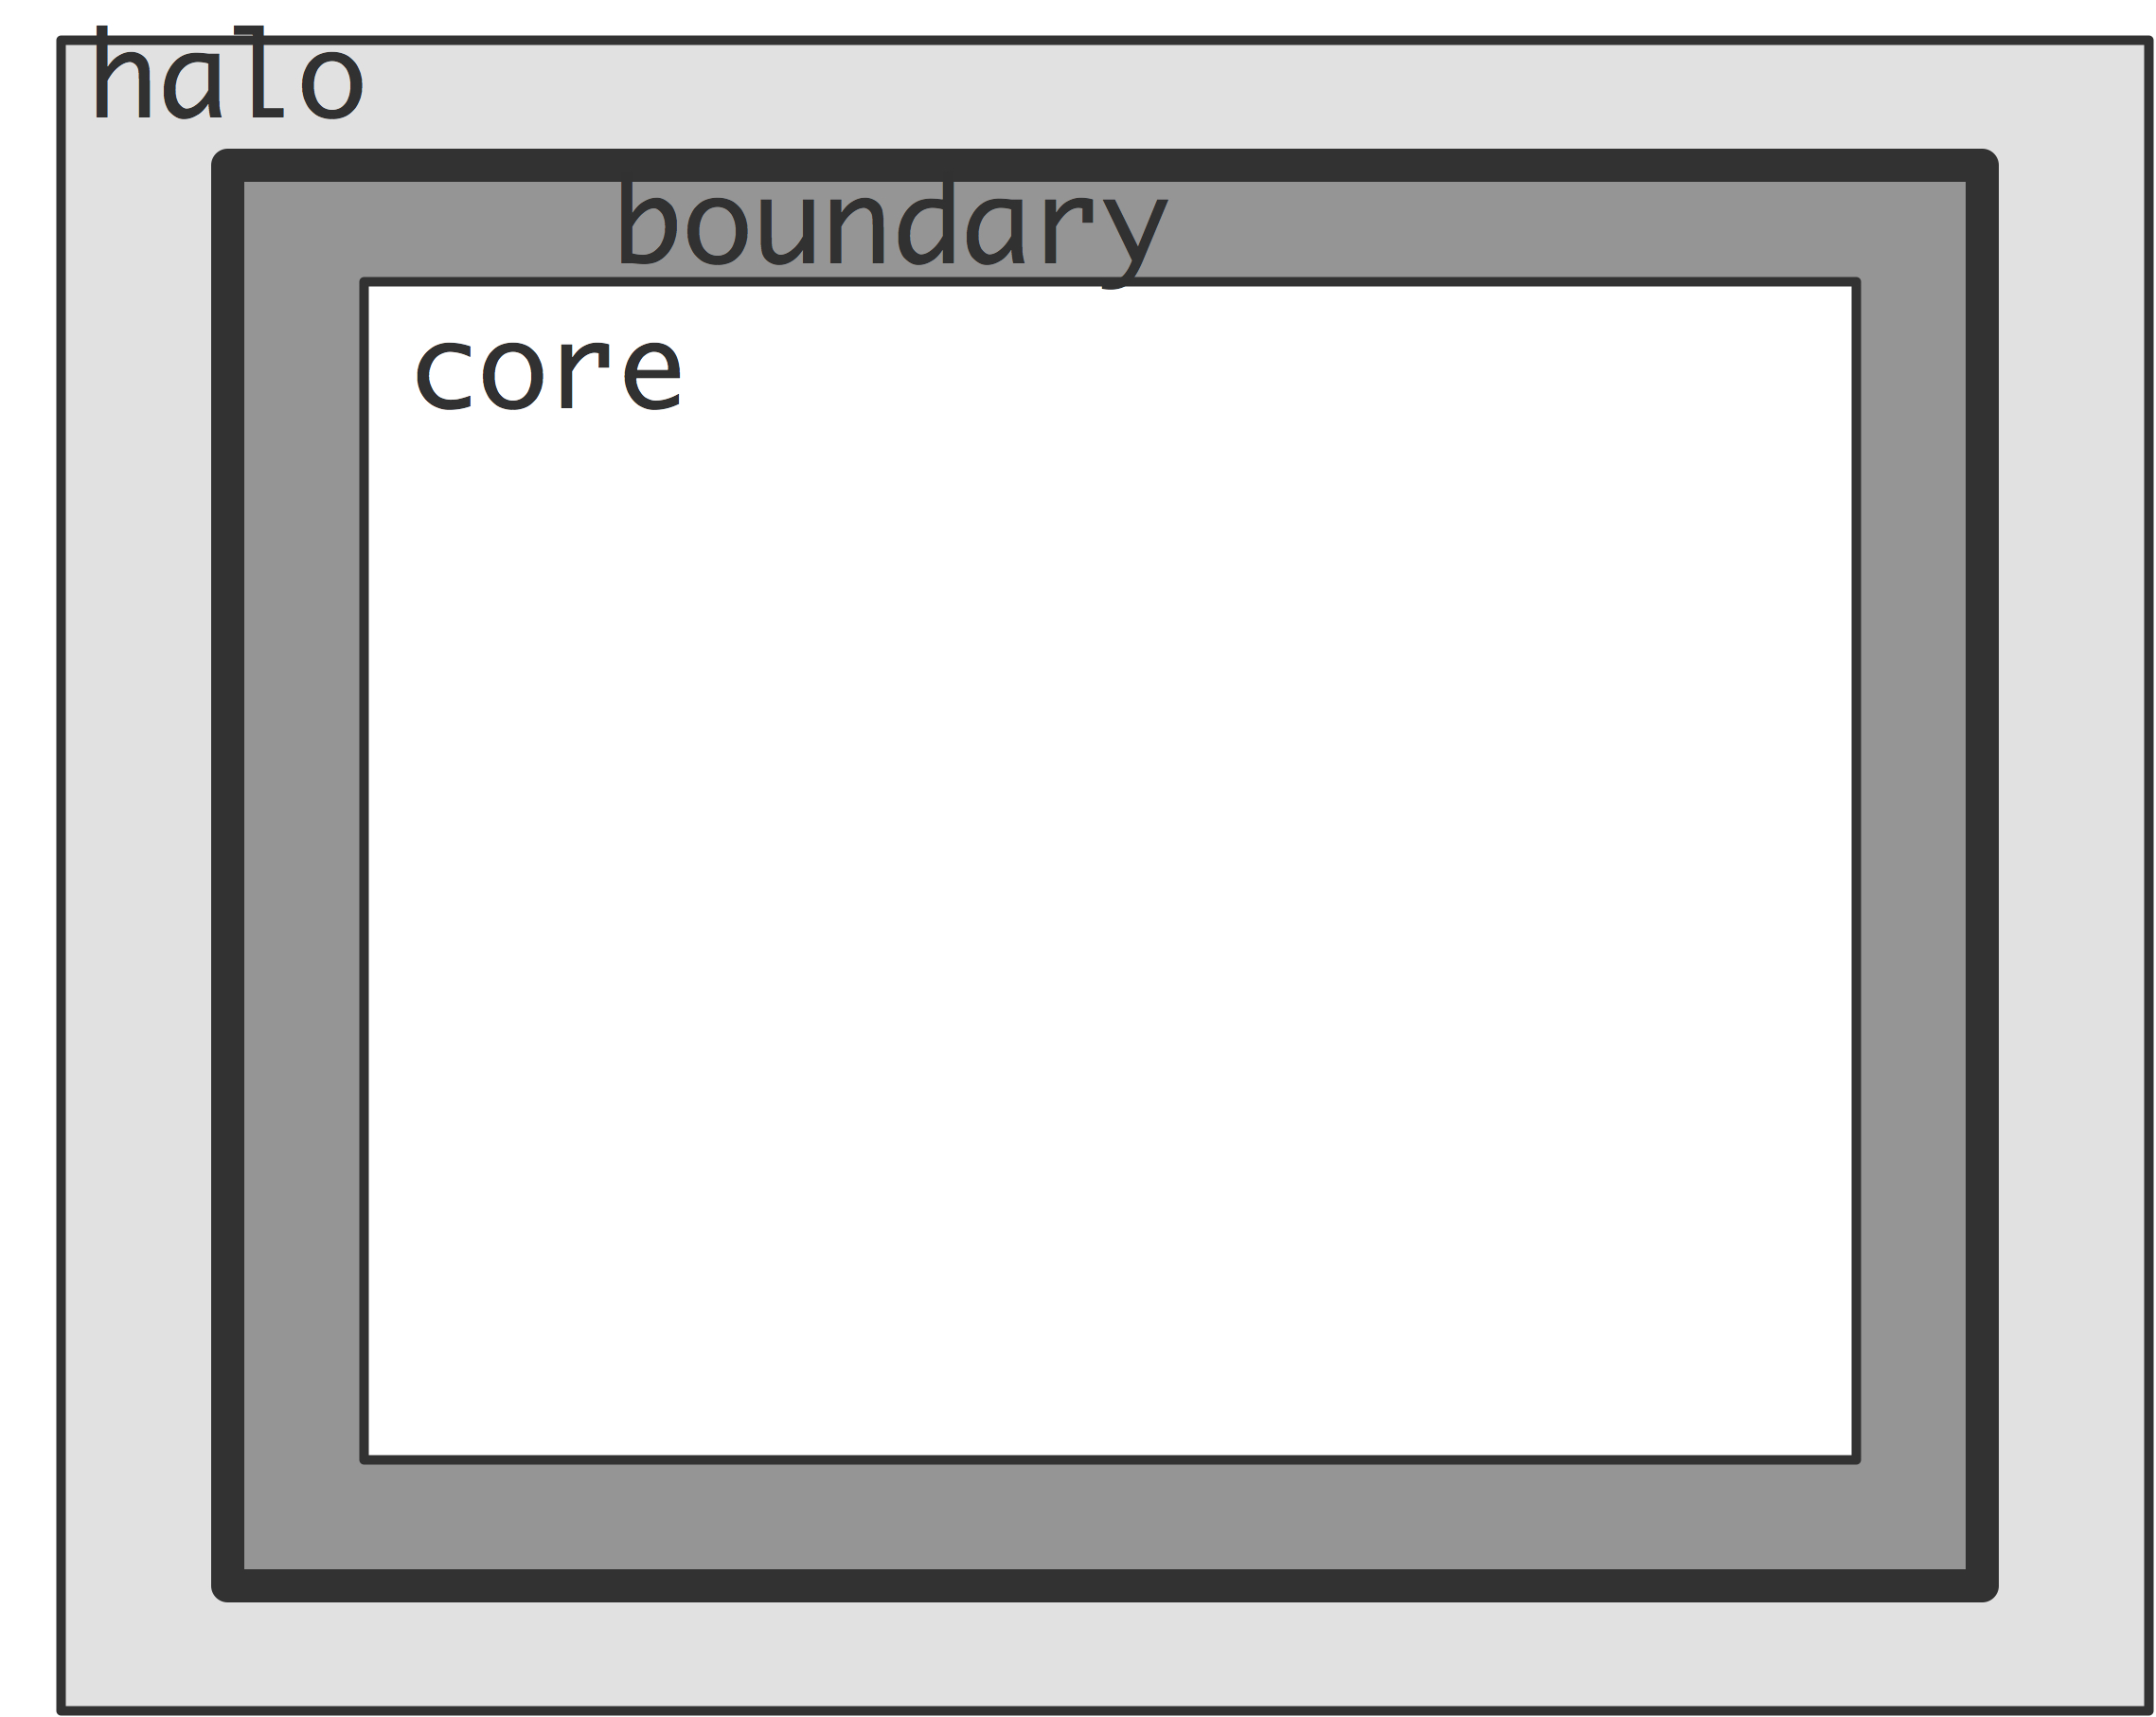
\includegraphics[scale=.08]{core-update}
\end{wrapfigure}
%
As an example, let's look at \indextermbus{halo}{update}.
The array~\n{A} is updated using the local values and the halo
that comes from bordering processors, either through Put or Get operations.

In a first version we separate computation and communication.
Each iteration has two fences. Between the two fences in the loop body
we do the \indexmpishow{MPI_Put} operation; between the second and and first one
of the next iteration there is only computation, so we add the
\n{NOPRECEDE} and \n{NOSUCCEED} assertions. (For much more about
assertions, see section~\ref{sec:mpi-assert} below.)
The \n{NOSTORE} assertion
states that the local window was not updated: the Put operation only
works on remote windows.
\begin{lstlisting}
for ( .... ) {
  update(A); 
  MPI_Win_fence(MPI_MODE_NOPRECEDE, win); 
  for(i=0; i < toneighbors; i++) 
    MPI_Put( ... );
  MPI_Win_fence((MPI_MODE_NOSTORE | MPI_MODE_NOSUCCEED), win); 
  }
\end{lstlisting}

Next, we split the update in the core part, which can be done purely
from local values, and the boundary, which needs local and halo
values. Update of the core can overlap the communication of the halo.
\begin{lstlisting}
for ( .... ) {
  update_boundary(A); 
  MPI_Win_fence((MPI_MODE_NOPUT | MPI_MODE_NOPRECEDE), win); 
  for(i=0; i < fromneighbors; i++) 
    MPI_Get( ... );
  update_core(A); 
  MPI_Win_fence(MPI_MODE_NOSUCCEED, win); 
  }
\end{lstlisting}
The \n{NOPRECEDE} and \n{NOSUCCEED} assertions still hold, but the
\n{Get} operation implies that instead of \n{NOSTORE} in the
second fence, we use \n{NOPUT} in the first.

\Level 1 {Accumulate}

A~third one-sided routine
is \indexmpishow{MPI_Accumulate} which does a reduction operation on the results
that are being put:

\mpiRoutineRef{MPI_Accumulate}

Accumulate is a reduction with remote result. As with \indexmpishow{MPI_Reduce}, the 
order in which the operands are accumulated is undefined. 
The same predefined operators are available, but no
user-defined ones. There is one extra operator: \indexmpidef{MPI_REPLACE},
this has the effect that only the last result to arrive is retained.

\begin{exercise}
  Implement an `all-gather' operation using one-sided communication:
  each processor stores a single number, and you want each processor
  to build up an array that contains the values from all
  processors. Note that you do not need a special case for a processor
  collecting its own value: doing `communication' between a processor
  and itself is perfectly legal.
\end{exercise}

\begin{exercise}
  \label{ex:countdown}

  Implement a shared counter:
  \begin{itemize}
  \item One process maintains a counter;
  \item Iterate: all others at random moments update this counter.
  \item When the counter is no longer positive, everyone stops iterating.
  \end{itemize}
  The problem here is data synchronization: does everyone see the
  counter the same way?
\end{exercise}

\Level 1 {Ordering and coherence of RMA operations}

There are few guarantees about what happens inside one epoch.
\begin{itemize}
\item No ordering of Get and Put/Accumulate operations: if you do
  both, there is no guarantee whether the Get will find the value
  before or after the update.
\item No ordering of multiple Puts. It is safer to do an Accumulate.
\end{itemize}
The following operations are well-defined inside one epoch:
\begin{itemize}
\item Instead of multiple Put operations, use Accumulate with
  \indexmpishow{MPI_REPLACE}.
\item \indexmpishow{MPI_Get_accumulate} with
  \indexmpishow{MPI_NO_OP} is safe.
\item Multiple Accumulate operations from one origin are done in
  program order by default. To allow reordering, for instance to have
  all reads happen after all writes, use the info parameter
  when the window is created; section~\ref{sec:window-info}.
\end{itemize}

\Level 1 {Request-based operations}

Analogous to \indexmpishow{MPI_Isend} there are request based one-sided operations:
%
\mpiRoutineRef{MPI_Rput}
%
and similarly \indexmpishow{MPI_Rget} and \indexmpishow{MPI_Raccumulate}.

These only apply to passive target synchronization.
Any \indexmpishow{MPI_Win_flush...} call also terminates these transfers.

\Level 1 {Assertions}
\label{sec:mpi-assert}

The \indexmpishow{MPI_Win_fence} call, as well \indexmpishow{MPI_Win_start} and such, take an argument
through which assertions can be passed about the activity before, after, and during the epoch.
The value zero is always allowed, by you can make your program more efficient by specifying
one or more of the following, combined by bitwise OR in C/C++ or
\n{IOR} in Fortran.

\begin{itemize}
\item[\indexmpishow{MPI_Win_start}] Supports the option:
  \begin{itemize}
    \item[\indexmpishow{MPI_MODE_NOCHECK}] the matching calls to \n{MPI_WIN_POST} have already
    completed on all target processes when the call to \n{MPI_WIN_START} is
    made. The nocheck option can be specified in a start call if and
    only if it is specified in each matching post call. This is similar
    to the optimization of ``ready-send'' that may save a handshake when
    the handshake is implicit in the code. (However, ready-send is
    matched by a regular receive, whereas both start and post must
    specify the nocheck option.)
  \end{itemize}
\item[\indexmpishow{MPI_Win_post}] supports the following options:
  \begin{itemize}
  \item[\indexmpishow{MPI_MODE_NOCHECK}] the matching calls to \n{MPI_WIN_START} have not
    yet occurred on any origin processes when the call to \n{MPI_WIN_POST}
    is made. The nocheck option can be specified by a post call if and
    only if it is specified by each matching start call.
  \item[\indexmpishow{MPI_MODE_NOSTORE}] the local window was not updated by local
    stores (or local get or receive calls) since last
    synchronization. This may avoid the need for cache synchronization
    at the post call.
  \item[\indexmpishow{MPI_MODE_NOPUT}] the local window will not be updated by put or
    accumulate calls after the post call, until the ensuing (wait)
    synchronization. This may avoid the need for cache synchronization
    at the wait call.
  \end{itemize}
\item[\indexmpishow{MPI_Win_fence}] supports the following options:
  \begin{itemize}
  \item[\indexmpishow{MPI_MODE_NOSTORE}] the local window was not updated by local
    stores (or local get or receive calls) since last synchronization.
  \item[\indexmpishow{MPI_MODE_NOPUT}] the local window will not be updated by put or
    accumulate calls after the fence call, until the ensuing (fence)
    synchronization.
  \item[\indexmpishow{MPI_MODE_NOPRECEDE}] the fence does not complete any sequence of
    locally issued RMA calls. If this assertion is given by any
    process in the window group, then it must be given by all
    processes in the group.
  \item[\indexmpishow{MPI_MODE_NOSUCCEED}] the fence does not start any
    sequence of locally issued RMA calls. If the assertion is given by
    any process in the window group, then it must be given by all
    processes in the group.
  \end{itemize}
\item[\indexmpishow{MPI_Win_lock}] supports the following option:
  \begin{itemize}
    \item[\indexmpishow{MPI_MODE_NOCHECK}] no other process holds, or will attempt to
    acquire a conflicting lock, while the caller holds the window
    lock. This is useful when mutual exclusion is achieved by other
    means, but the coherence operations that may be attached to the
    lock and unlock calls are still required.
  \end{itemize}
\end{itemize}

\Level 1 {More active target synchronization}
\label{sec:ref:post-wait}

The `fence' mechanism (section~\ref{sec:fence}) uses a global synchronization on the
communicator of the window. As such it is good for applications where
the processes are largely synchronized, but it may 
lead to performance inefficiencies if processors are not in step which each other. 
There is a mechanism that is more fine-grained, by using synchronization only 
on a processor \indexterm{group}. This takes four different calls, two for starting
and two for ending the epoch, separately for target and origin.
\begin{figure}[ht]
  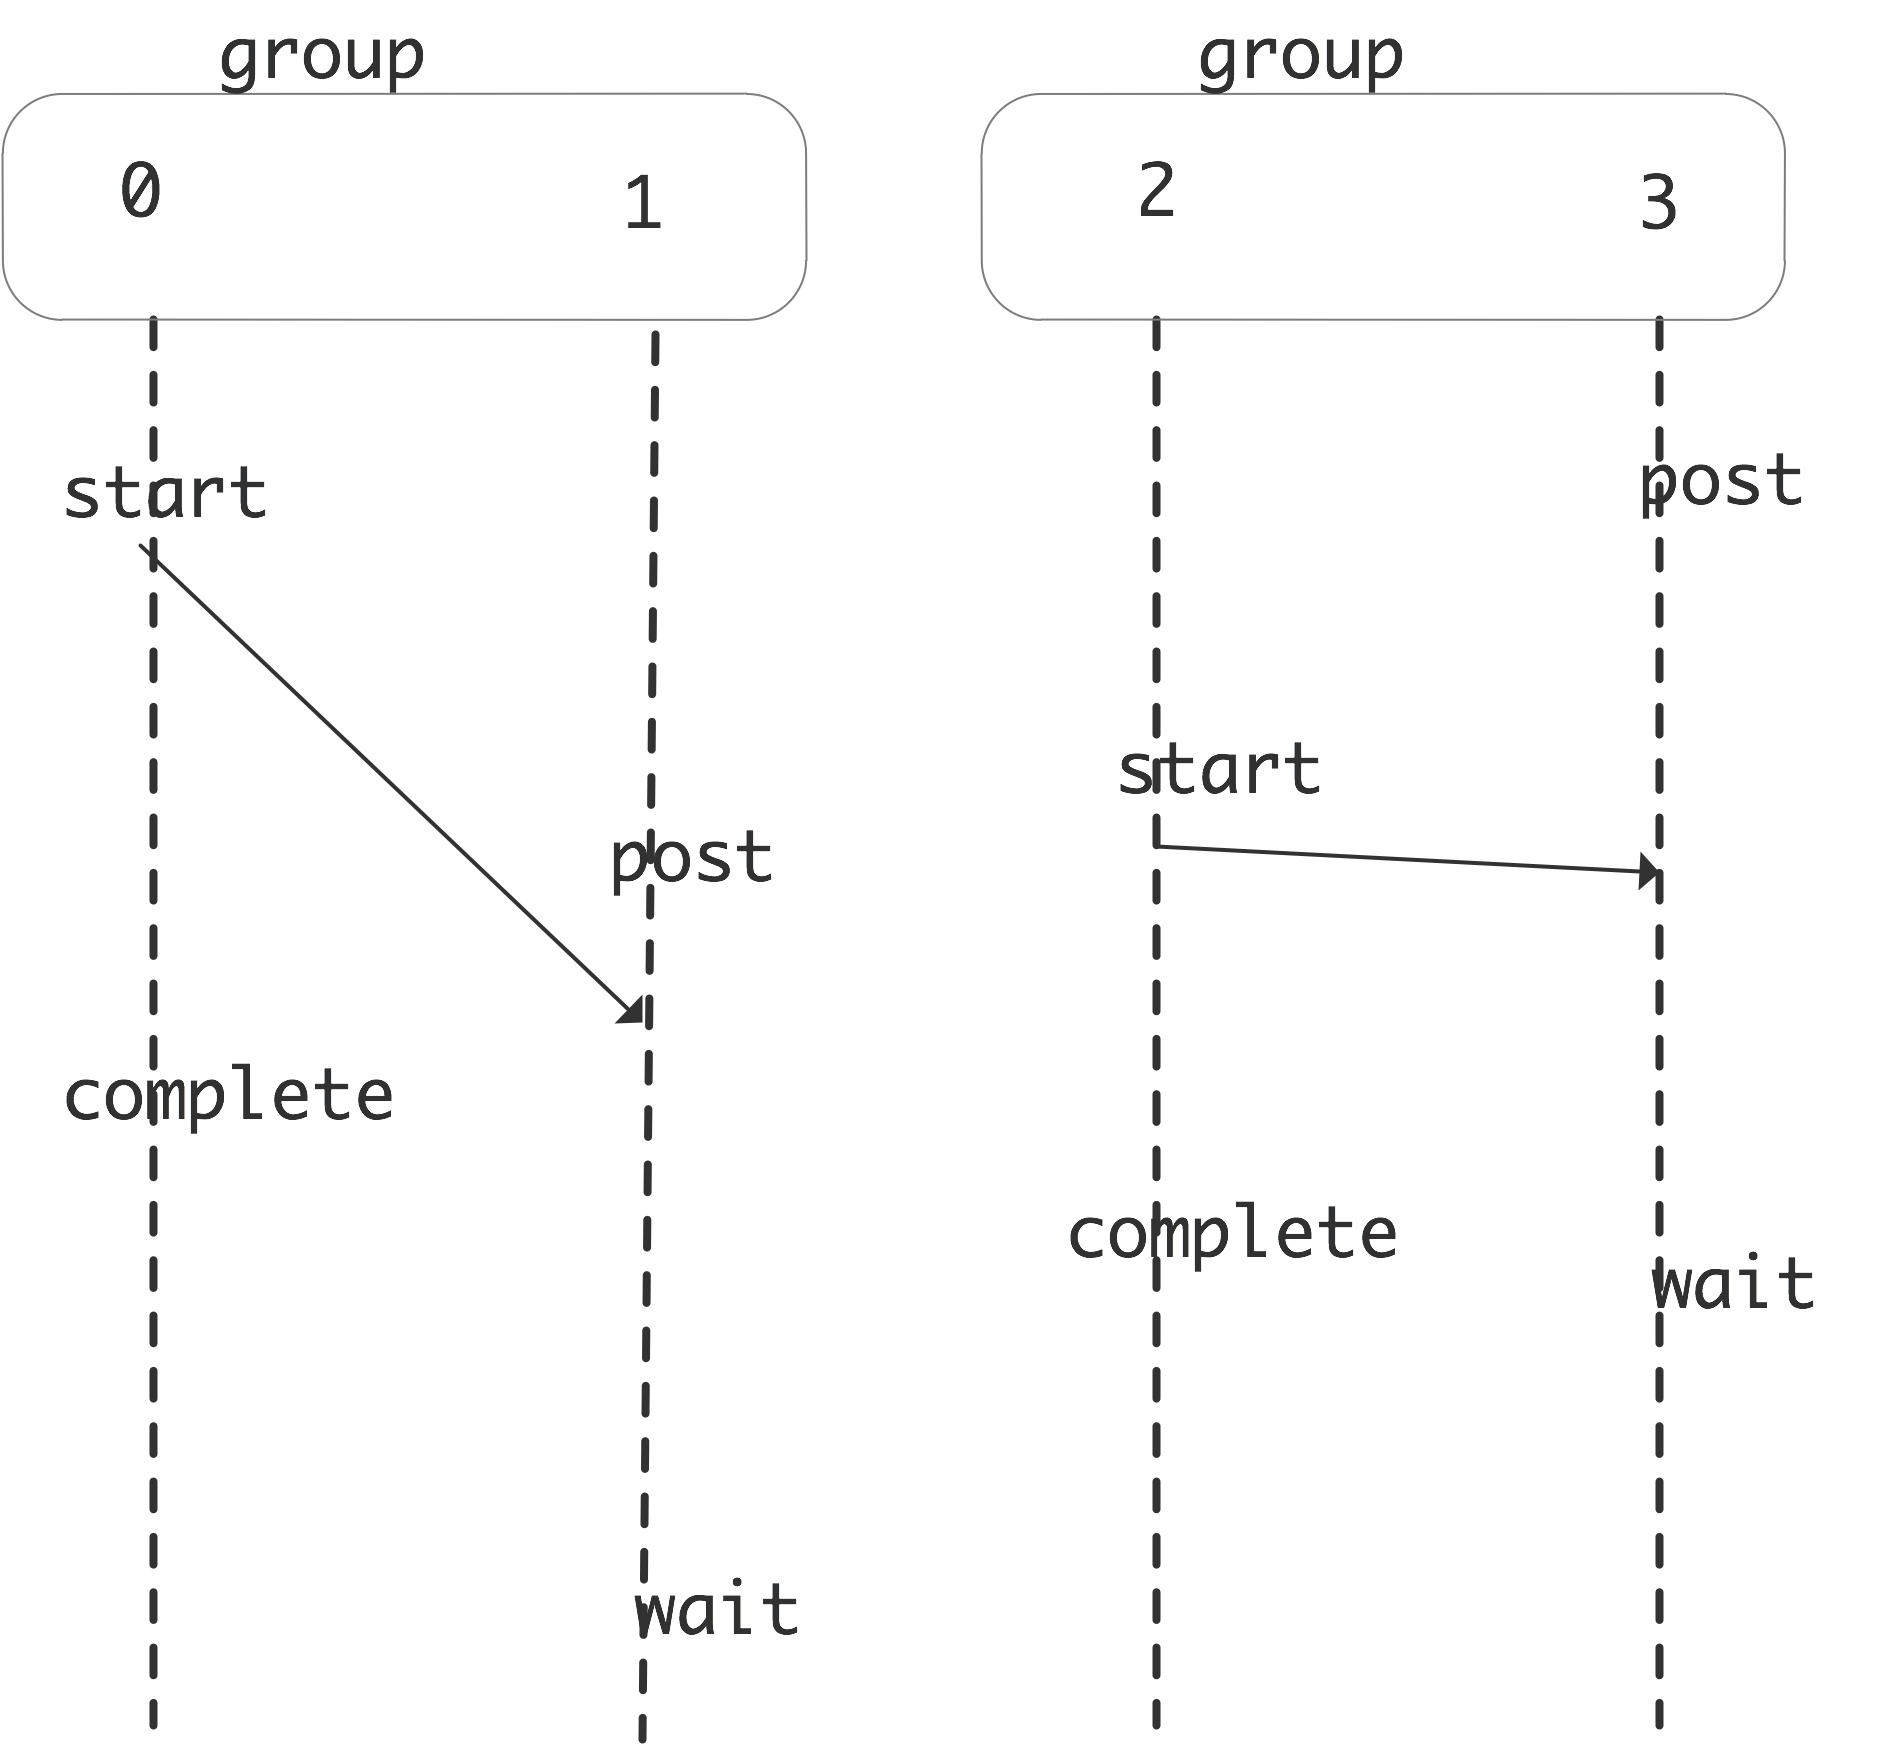
\includegraphics[scale=.1]{postwait}
  \caption{Window locking calls in fine-grained active target synchronization}
  \label{fig:postwait}
\end{figure}

You start and complete an \indextermsub{exposure}{epoch} with%
\indexmpi{MPI_Win_post}\indexmpi{MPI_Win_wait}:
\begin{lstlisting}
int MPI_Win_post(MPI_Group group, int assert, MPI_Win win)
int MPI_Win_wait(MPI_Win win)
\end{lstlisting}
In other words, this turns your window into the \indexterm{target} for a remote access.

You start and complete an \indextermsub{access}{epoch} with%
\indexmpi{MPI_Win_start}\indexmpi{MPI_Win_complete}:
\begin{lstlisting}
int MPI_Win_start(MPI_Group group, int assert, MPI_Win win)
int MPI_Win_complete(MPI_Win win)
\end{lstlisting}
In other words, these calls border the access to a remote window, with the current processor
being the \indexterm{origin} of the remote access.

In the following snippet a single processor puts data on one
other. Note that they both have their own definition of the group, and
that the receiving process only does the post and wait calls.
%
\cverbatimsnippet[examples/mpi/c/postwaittwo.c]{postwaittwo}

Both pairs of operations declare a
\indextermbus{group of}{processors}; see section~\ref{sec:comm-group}
for how to get such a group from a communicator.
On an origin processor you would specify a group that includes the targets
you will interact with, on a target processor you specify a group
that includes the possible origins.

\Level 1 {Atomic operations}
\label{sec:mpi-atomic}

One-sided calls are said to emulate shared memory in MPI, but 
the put and get calls are not enough for certain scenarios with shared
data. Consider the scenario where:
\begin{itemize}
\item One process stores a table of work descriptors, and a pointer to
  the firt unprocessed descriptor;
\item Each process reads the pointer, reads the corresponding
  descriptor, and increments the pointer; and
\item A process that has read a descriptor then executes the
  corresponding task.
\end{itemize}
The problem is that reading and updating the pointer is not an
\indexterm{atomic operation}, so
it is possible that multiple processes get hold of the same value;
conversely, multiple updates of the pointer may lead to work
descriptors being skipped. These inconsistent views of the data are
called a \indexterm{race condition}.

In \indextermbus{MPI}{3} some atomic routines have been added.
Both \indexmpi{MPI_Fetch_and_op} and \indexmpi{MPI_Get_accumulate}
atomically retrieve data from the window indicated,
and apply an operator, combining the data on the target
with the data on the origin.
%
\mpiRoutineRef{MPI_Fetch_and_op}
%
\mpiRoutineRef{MPI_Get_accumulate}

Both routines perform the same operations: return data before the
operation, then atomically update data on the target, but
\indexmpishow{MPI_Get_accumulate} is more flexible in data type
handling. The more simple routine, \indexmpishow{MPI_Fetch_and_op},
which operates on only a single element,
allows for faster implementations, in particular through hardware support.

\begin{exercise}
  \label{ex:countdownop}
  Redo exercise~\ref{ex:countdown} using \indexmpishow{MPI_Fetch_and_op}. The
  problem is again to make sure all processes have the same view of
  the shared counter.

  Does it work to make the fetch-and-op conditional? Is there a way to
  do it unconditionally? What should the `break' test be, seeing that
  multiple processes can update the counter at the same time?
\end{exercise}

\begin{example}
  A root process has a table of data; the other processes do 
  atomic gets and update of that data using
  \indexterm{passive target synchronization} through \indexmpishow{MPI_Win_lock}.
  %
  \cverbatimsnippet[examples/mpi/c/fetchop.c]{fetchop}
  %
  \pverbatimsnippet{fetchopp}
\end{example}

Finally, \indexmpishow{MPI_Compare_and_swap} swaps the origin and
target data if the target data equals some comparison value.
%
\mpiRoutineRef{MPI_Compare_and_swap}

\Level 0 {Passive target synchronization}
\label{sec:passive-sync}

In \indexterm{passive target synchronization} only the origin is
actively involved: the target makes no calls whatsoever.
This means that the origin process remotely locks the window
on the target, performs a one-sided transfer, and releases the window
by unlocking it again.

During access epoch, also called an
\indextermsubdef{passive target}{epoch} in this case,
a~process can initiate and finish a one-sided
transfer.
\begin{lstlisting}
If (rank == 0) {
  MPI_Win_lock (MPI_LOCK_EXCLUSIVE, 1, 0, win);
  MPI_Put (outbuf, n, MPI_INT, 1, 0, n, MPI_INT, win);
  MPI_Win_unlock (1, win);
}
\end{lstlisting}
The two lock types are:
\begin{itemize}
\item \indexmpishow{MPI_LOCK_SHARED} which should be used for \n{Get}
  calls: since multiple processors are allowed to read from a window
  in the same epoch, the lock can be shared.
\item \indexmpishow{MPI_LOCK_EXCLUSIVE} which should be used for
  \n{Put} and \n{Accumulate} calls: since only one processor is
  allowed to write to a window during one epoch, the lock should be
  exclusive.
\end{itemize}
These routines make MPI behave like a shared memory system; the
instructions between locking and unlocking the window effectively
become \indexterm{atomic operations}.
%
\mpiRoutineRef{MPI_Win_lock}

To lock the windows of all processes in the group of the windows, use
\indexmpishow{MPI_Win_lock_all}:
%
\mpiRoutineRef{MPI_Win_lock_all}

To unlock a window, use \indexmpishow{MPI_Win_unlock} and
\indexmpishow{MPI_Win_unlock_all}.

\mpiRoutineRef{MPI_Win_unlock} % includes unlock_all

\Level 1 {Completion and consistency}

In one-sided transfer one should keep straight the multiple instances
of the data, and the various \indextermdef{completion}s that effect
their \emph{consistency}\index{window!consistency}.
\begin{itemize}
\item The user data. This is the buffer that is passed to a \n{Put} or
  \n{Get} call. For instance, after a \n{Put} call, but still in an
  access epoch, the user buffer is not safe to reuse. Making sure the
  buffer has been transferred is called \indextermsub{local}{completion}.
\item The window data. While this may be publicly accessible, it is
  not necessarily always consistent with internal copies.
\item The remote data. Even a successful \n{Put} does not guarantee
  that the other process has received the data. A~successful transfer
  is a \indextermsub{remote}{completion}.
\end{itemize}

You can force the remote completition, that is, update on the target
with
\indexmpishow{MPI_Win_unlock} or some variant of it, concluding the
epoch.

There is also
\indexmpishow{MPI_Win_flush} or
\indexmpishow{MPI_Win_flush_all}, which has to come inside the
\indextermsub{passive target}{epoch}.
%
\mpiRoutineRef{MPI_Win_flush}

Local completion, again: during the epoch, is done with
with \indexmpishow{MPI_Win_flush_local} or
\indexmpishow{MPI_Win_flush_local_all}.
After these, buffers involved in the call can be reused.
%
\mpiRoutineRef{MPI_Win_flush_local}

Finally, there is \indexmpidef{MPI_Win_sync} which synchronizes
private and public copies of the window.

\Level 1 {Atomic shared memory operations}

The above example is of limited use.
Suppose processor zero has a data structure \n{work_table}
with items that need to be processed. A~counter \n{first_work}
keeps track of the lowest numbered item that still needs processing.
You can imagine the following
\indexterm{master-worker} scenario:
\begin{itemize}
\item Each process connects to the master,
\item inspects the \n{first_work} variable,
\item retrieves the corresponding work item, and
\item increments the \n{first_work} variable.
\end{itemize}
It is important here to avoid a \indexterm{race condition}
(see section \HPSCref{sec:shared-lock}) that would result
from a second process reading the \n{first_work} variable 
before the first process could have updated it. Therefore, the reading
and updating needs to be an \indexterm{atomic operation}.

Unfortunately, you can not have a put and get call in the same access
epoch. For this reason, MPI version~3 has added certain atomic
operations, such as \indexmpishow{MPI_Fetch_and_op}.

\begin{exercise}
  \label{ex:onesidedbuild}
  \begin{itemize}
  \item
    Let each process have an empty array of sufficient length and a
    stack pointer that maintains the first free location.
  \item
    Now let each process randomly put data in a free location of another
    process' array.
  \item Use window locking. (Why is active target synchronization not possible?)
  \end{itemize}
\end{exercise}

\Level 0 {Details}

\Level 1 {More about window memory}
\label{sec:win-model}

In section~\ref{sec:win-alloc} we looked at simple ways to create a
window and its memory.

It is also possible to have windows where the size is dynamically set.
%
\mpiRoutineRef{MPI_Win_create_dynamic}
%
Memory is attached to the window:
%
\mpiRoutineRef{MPI_Win_attach}
%
and its inverse:
%
\mpiRoutineRef{MPI_Win_detach}

You may now think that the window memory is the same as the buffer you
pass to \indexmpishow{MPI_Win_create} or that you get from
\indexmpishow{MPI_Win_allocate}. This is not necessarily true, and the
actual state of affairs is called the \emph{memory
  model}\index{window!memory!model}. There are two memory models:
\begin{itemize}
\item Under the \emph{unified}\index{window!memory!unified} memory
  model, the buffer in process space is indeed the window memory. This
  means that after \emph{completion}\index{epoch!completion} of an
  epoch you can read the window contents from the buffer.
\item Under the \emph{separate}\index{window!memory!separate} memory
  model, the buffer in process space is the
  \indextermsub{private}{window} and the target of put/get operations
  is the \indextermsub{public}{window} and the two are not the same
  and are not kept coherent. Under this model, you need to do an
  explicit get to read the window contents.
\end{itemize}
See also section~\ref{sec:win-attr}.

\Level 1 {Window usage hints}
\label{sec:window-info}

The following keys can be passed as info argument:
\begin{itemize}
\item \indexmpishow{no_locks}: if set to true, passive target synchronization
  (section~\ref{sec:passive-sync}) will not be used on this window.
\item \indexmpishow{accumulate_ordering}: a comma-separated list of
  the keywords \indextermtt{rar}, \indextermtt{raw},
  \indextermtt{war}, \indextermtt{waw} can be specified. This
  indicates that reads or writes from \indexmpishow{MPI_Accumulate} or
  \indexmpishow{MPI_Get_accumulate} can be reordered, subject to
  certain constraints.
\item \indexmpishow{accumulate_ops}: the value \indexmpishow{same_op}
  indicates that concurrent Accumulate calls use the same operator;
  \indexmpishow{same_op_no_op} indicates the same operator or
  \indexmpishow{MPI_NO_OP}.
\end{itemize}

\Level 1 {Window information}
\label{sec:win-attr}

The \indexmpishow{MPI_Info} parameter can be used to pass implementation-dependent 
information; see section~\ref{sec:mpi-info}.

A number of attributes are stored with a window when it is created.

Obtaining a pointer to the start of the window area:
\begin{lstlisting}
void *base;
MPI_Win_get_attr(win, MPI_WIN_BASE, &base, &flag)  
\end{lstlisting}

Obtaining the size and \indextermbus{window}{displacement unit}:
\begin{lstlisting}
MPI_Aint *size;
MPI_Win_get_attr(win, MPI_WIN_SIZE, &size, &flag), 
int *disp_unit;
MPI_Win_get_attr(win, MPI_WIN_DISP_UNIT, &disp_unit, &flag), 
\end{lstlisting}

The type of create call used:
\begin{lstlisting}
int *create_kind;
MPI_Win_get_attr(win, MPI_WIN_CREATE_FLAVOR, &create_kind, &flag)
\end{lstlisting}
with possible values:
\begin{itemize}
\item \indexmpishow{MPI_WIN_FLAVOR_CREATE} if the window was create
  with \indexmpishow{MPI_Win_create};
\item \indexmpishow{MPI_WIN_FLAVOR_ALLOCATE} if the window was create
  with \indexmpishow{MPI_Win_allocate};
\item \indexmpishow{MPI_WIN_FLAVOR_DYNAMIC} if the window was create
  with \indexmpishow{MPI_Win_create_dynamic}. In this case the base is
  \indexmpishow{MPI_BOTTOM} and the size is zero;
\item \indexmpishow{MPI_WIN_FLAVOR_SHARED} if the window was create
  with \indexmpishow{MPI_Win_allocate_shared};
\end{itemize}

The window model:
\begin{lstlisting}
int *memory_model;
MPI_Win_get_attr(win, MPI_WIN_MODEL, &memory_model, &flag);
\end{lstlisting}
with possible values:
\begin{itemize}
\item \indexmpishow{MPI_WIN_SEPARATE},
\item \indexmpishow{MPI_WIN_UNIFIED},
\end{itemize}

Get the group of processes associated with a window:
\begin{verbatim}
int MPI_Win_get_group(MPI_Win win, MPI_Group *group) 
MPI_Win_get_group(win, group, ierror) 
TYPE(MPI_Win), INTENT(IN) :: win 
TYPE(MPI_Group), INTENT(OUT) :: group 
INTEGER, OPTIONAL, INTENT(OUT) :: ierror
\end{verbatim}

\begin{verbatim}
int MPI_Win_set_info(MPI_Win win, MPI_Info info)
MPI_Win_set_info(win, info, ierror)
TYPE(MPI_Win), INTENT(IN) :: win
TYPE(MPI_Info), INTENT(IN) :: info
INTEGER, OPTIONAL, INTENT(OUT) :: ierror

int MPI_Win_get_info(MPI_Win win, MPI_Info *info_used)
MPI_Win_get_info(win, info_used, ierror)
TYPE(MPI_Win), INTENT(IN) :: win
TYPE(MPI_Info), INTENT(OUT) :: info_used
INTEGER, OPTIONAL, INTENT(OUT) :: ierror
\end{verbatim}

\Level 0 {Implementation}
\index{communication!one-sided, implementation of|(}

You may wonder how one-sided communication is realized\footnote{For
  more on this subject, see~\cite{thakur:ijhpca-sync}.}. Can a processor
somehow get at another processor's data? Unfortunately, no.

Active target synchronization is implemented in terms of two-sided communication.
Imagine that the first fence operation does nothing, unless it concludes prior
one-sided operations. The Put and Get calls do nothing involving communication,
except for marking with what processors they exchange data.
The concluding fence is where everything happens: first a global operation
determines which targets need to issue send or receive calls, then the
actual sends and receive are executed.

\begin{exercise}
  Assume that only Get operations are performed during an epoch. 
  Sketch how these are translated to send/receive pairs. 
  The problem here is how the senders find out that they need to send.
  Show that you can solve this with an \indexmpishow{MPI_Reduce_scatter} call.
\end{exercise}

The previous paragraph noted that a collective operation was necessary
to determine the two-sided traffic. Since collective operations induce
some amount of synchronization, you may want to limit this.

\begin{exercise}
  Argue that the mechanism with window post/wait/start/complete operations
  still needs a collective, but that this is less burdensome.
\end{exercise}

Passive target synchronization needs another mechanism entirely.  Here
the target process needs to have a background task (process, thread,
daemon,\ldots) running that listens for requests to lock the
window. This can potentially be expensive.

\index{communication!one-sided, implementation of|)}
\index{communication!one-sided|)}

